\chapter{Конструкторский раздел}
В этом разделе приводится подробное описание разрабатываемого метода, выделяются основные его компоненты, описываются метрики, оценивающие метод. 
В выводах аналитической части предлагается разработать новый метод прогнозирования результатов теннисных матчей. Новый метод будет включать в себя построение модели на основе численных статистических данных, а так же текстовых данных.

\section{Структура программного комплекса}
\begin{figure}[!h]
	\centering
	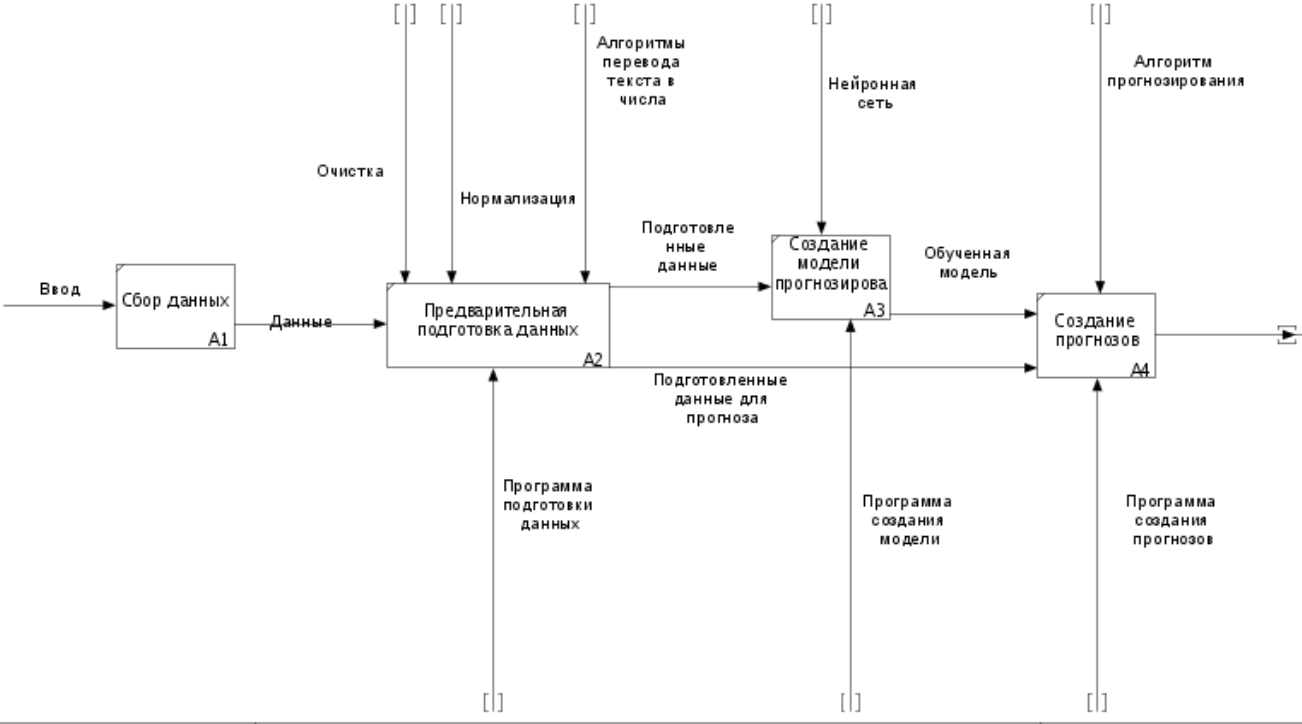
\includegraphics[width=.9\textwidth]{diagrams/img/main_img_cut.png}
	\caption{Общая схема программного комплекса}
	\label{fig08}
\end{figure}
Для того, чтобы создать модель прогнозирования, необходимы данные. Статистические и текстовые данные собираются с различных источников, сопоставляются и приводятся в формат, пригодный для чтения программой подготовки данных. Программы подготовки выполняют следующие действия:
\begin{itemize}
	\item Нормализуют статистические данные
	\item Преобразуют текстовые данные в числовые
	\item Выбирают наиболее полезные статистические данные
	\item Объединяют статистические данные и преобразованные текстовые в один датасет
\end{itemize}
Результатом предварительной подготовки данных является нормализованный числовой набор данных, разделенный на две части - обучающую и тестовую.
Обучающая выборка используется программой создания модели.
После создания модели, она проверяется на данных, которые не участвовали в обучение, - тестовой выборке.
Полученная модель может использоваться в программе прогнозирования отдельных матчей.
\section{Обработка текстовых данных}

Работа осуществляется с текстами только на английском языке.
Для того чтобы  преобразовать текстовые данные в числовое представление, нужно выполнить следующие действия:

\begin{itemize}
	\item Удалить все нерелевантные символы (например, любые символы, не относящиеся к цифро-буквенным).
	\item Разделить текст на отдельные слова
	\item Удалить нерелевантные слова — например,  гиперссылки.
	\item Перевести все символы в нижний регистр для того, чтобы слова «привет», «Привет» и «ПРИВЕТ» считались одним и тем же словом.

	\item Произвести лемматизацию, т. е. сведения различных форм одного слова к словарной форме (например, «машина» вместо «машиной», «на машине», «машинах» и пр.)
	\item Удалить слова, не несущих самостоятельной смысловой нагрузки. Например, артиклей в английском языке.
	\item Произвести стемминг текста, т.е. заменить исходные слова их основами.

\end{itemize}


\section{Определение тональности текста}
Используем численную метрику тональности текста для её добавления в численный набор данных. Для этот используем вышеописанный метод word2vec с алгоритмом CBOW с размером контекста 1\ref{fig09}.
\begin{figure}[!h]
	\centering
	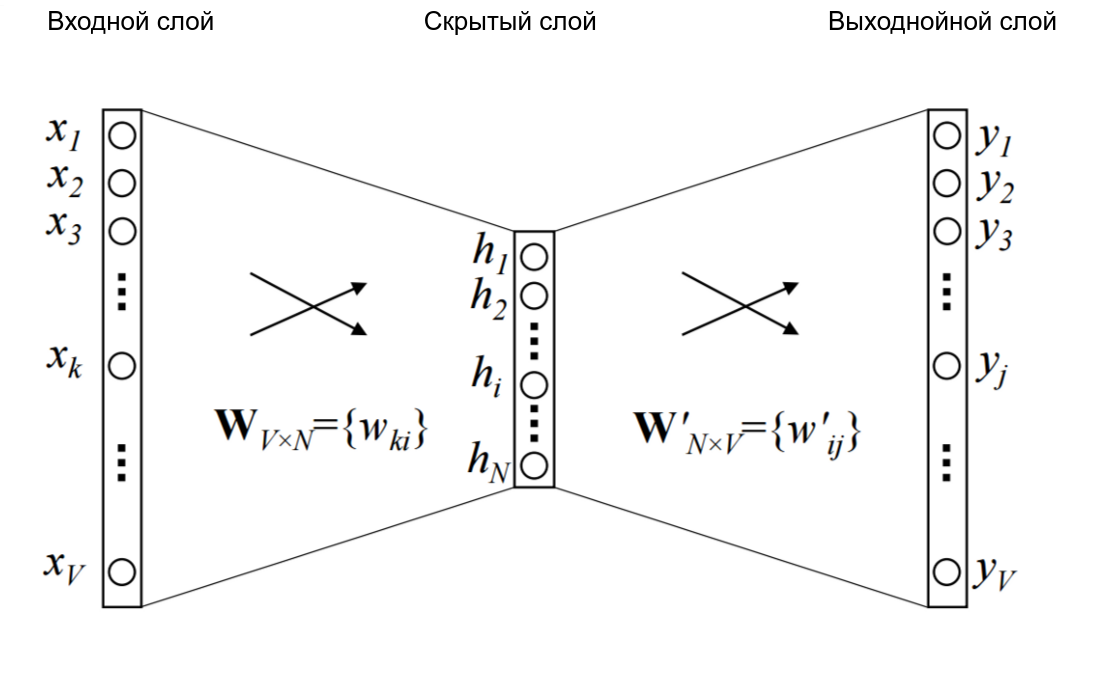
\includegraphics[scale=0.4]{master_img/cbow_model2_edited.png}
	\caption{Архитектура нейронной сети word2vec CBOW с размером контекста 1}
	\label{fig09}
\end{figure}
 Первоначально каждое слово в словаре – случайный N-мерный вектор. Во время обучения алгоритм формирует оптимальный вектор для каждого слова с помощью метода CBOW. После обучения модели на размеченных данных на выходе получаем обученную модель. Использование модели для анализа конкретного слова даёт на выходе некоторый вектор значений фиксированного размера.
 Для каждого текста усредняем вектор вероятностей полученных слов.
 \begin{center}
 	
 \begin{lstlisting}[language=python,,escapeinside={(@}{@)},caption={Псевдокод алгоритма усреднения слов},   xleftmargin=.1\textwidth, xrightmargin=.1\textwidth] 
def buildWordVector(text, size):
	vec = np.zeros(size).reshape((1, size))
	count = 0.
	for word in text:
		try:
			vec += model[word].reshape((1, size))
			count += 1.
	 	except KeyError:
			continue
	if count != 0:
		vec /= count
	return vec

 \end{lstlisting}
 \end{center}

Для оценки тональности текста необходимо перевести полученные вектора слов в некое число.Для это понадобится бинарный классификатор, который на выходе будет давать вероятность того, что эмоция текста негативна.
Для этого применим вероятностный калибратор, основанный на логистической регрессии(sklearn.calibration.CalibratedClassifierCV из библиотеки scikit-learn).
Преобразуем наш исходный датасет в пары вида: вектор чисел - результат.
После этого обучим наш классификатор на новом наборе данный.
Обученный классификатор получает на вход некоторый текст, а на выходе даёт вероятность того,что текст является негативным.

\section{Нормализация данных}
Полученный набор оценок для каждого текста, а так же все статистические свойства нормализуем при помощи min-max нормализации по формуле \ref{mixmaxNorm}.
\section{Выбор оптимального набора параметров}
В нашем набора данных имеется набор статистических параметров, выберем из них N наиболее значимых параметров при помощи фильтр-метода Пирсона\ref{pearson}.
В нашем датасете имеется Y следующих параметров:
\begin{itemize}
	\item Рейтинг ATP 1-го игрока
	\item Рейтинг ATP 2-го игрока
	\item Где проводится турнир: в помещении или на улице
	\item Покрытие корта
	\item Максимальный коэффициент ставки на первого игрока
	\item Максимальный коэффициент ставки на второго игрока
	\item Средняя ставка на первого игрока
	\item Средняя ставка на второго игрока
	\item Стадия турнира
\end{itemize}

Из этого набора признаков необходимо выделить N оптимальных свойств(правила для выбора оптимального количества свойств являются открытым вопросом в современной науке\cite{Book32}), поэтому оптимальное количество слов подбирается эмпирическим путем).
\section{Прогнозирование результатов}
В нейронную сеть на вход подаются нормализованные статистические данные, совмещенные с текстовыми данными. Текстовые данные переведены в численный вид и нормализованы.
Нейронная сеть для прогнозирования результатов теннисных матчей имеет следующие параметры параметры:
\begin{itemize}
	\item Количество слоёв - 3, из них 2 скрытых.
	\item Количество нейронов на каждом слое: 64->32->1
	\item Функции активации по слоям:
	 линейный выпрямитель(англ. relu)->линейный выпрямитель->сигмоида
\end{itemize}
\begin{lstlisting}[language=python,,escapeinside={(@}{@)},caption={Псевдокод нейронной сети для осуществления прогнозов}, xleftmargin=.1\textwidth, xrightmargin=.1\textwidth] 

network = models.Sequential()
network.add(layers.Dense(units=64, activation='relu', input_shape=(len(features.columns),)))
network.add(layers.Dense(units=32, activation='relu'))
network.add(layers.Dense(units=1, activation='sigmoid'))

network.fit(train_features, train\_target, 
epochs=1000, verbose=0, batch\_size=128, 
validation_data=(test_features, test_target), callbacks=[es, mc]) 

\end{lstlisting}